\documentclass{article}
\usepackage{lingmacros}
\usepackage[danish]{babel}
\usepackage{enumitem}
\usepackage{lmodern}
\usepackage{float}
\usepackage[utf8]{inputenc}
\usepackage[T1]{fontenc}
\usepackage{color}
\usepackage{amssymb}
\usepackage{listings}
\usepackage{listingsutf8}
\usepackage{color} %red, green, blue, yellow, cyan, magenta, black, white
\definecolor{mygreen}{RGB}{28,172,0} % color values Red, Green, Blue
\definecolor{mylilas}{RGB}{170,55,241}
\lstset{literate=
  {æ}{{\ae}}{1} 
  {å}{{\aa}}{1} 
  {ø}{{\o}}{1} }
\usepackage{graphicx}
\usepackage[export]{adjustbox}
\usepackage{fullpage}
\lstset{basicstyle=\ttfamily,breaklines=true}
% \lstset{framextopmargin=50pt,frame=bottomline}
\lstset{
% numbers=left, 
% numberstyle=\small, 
% numbersep=8pt, 
frame = single, 
language=Pascal, 
framexleftmargin=15pt}
\usepackage[T1]{fontenc}
\usepackage[hidelinks]{hyperref}
 \usepackage{tree-dvips}
% \usepackage{biblatex}
% \usepackage[style=verbose,backend=bibtex]{biblatex}
% \bibliography{oeve1dsb.bib}
% \usepackage{sagetex}
\usepackage{amsmath}
% \usepackage{newpxtext,newpxmath}
\usepackage{courier}
\linespread{1.5}
\makeatletter
\renewcommand*\env@matrix[1][*\c@MaxMatrixCols c]{%
  \hskip -\arraycolsep
  \let\@ifnextchar\new@ifnextchar
  \array{#1}}
\makeatother
\title{E4DSA\\ Case projekt 2 – audio IIR notch filter}
\author{Team 8}
\def\emptyline{\vspace{12pt}}

\begin{document}
%\newcommand{\includecode}[2][c]{\lstinputlisting[caption=#2, escapechar=, style=custom#1]{#2}<!---->}
\lstset{language=Matlab,%
    %basicstyle=\color{red},
    breaklines=true,%
    morekeywords={matlab2tikz},
    keywordstyle=\color{blue},%
    morekeywords=[2]{1}, keywordstyle=[2]{\color{black}},
    identifierstyle=\color{black},%
    stringstyle=\color{mylilas},
    commentstyle=\color{mygreen},%
    showstringspaces=false,%without this there will be a symbol in the places where there is a space
    % numbers=left,%
    % numberstyle={\tiny \color{black}},% size of the numbers
    % numbersep=9pt, % this defines how far the numbers are from the text
    emph=[1]{for,end,break},emphstyle=[1]\color{red}, %some words to emphasise
    %emph=[2]{word1,word2}, emphstyle=[2]{style},    
  }
\maketitle
\tableofcontents
\newpage

\section{Data analyse}
\label{sec:Data analyse}

\subsection{Matlab kode}
\label{sec:matlab1}

\begin{lstlisting}
%% Indlæsning af data, samt skabelse af 2 dele af disse

load('vejecelle_data.mat');
x = vejecelle_data;

x1 = vejecelle_data(1:1000);
n1 = (1:1000);
N1 = 1000;
k1 = 0:N1-1;

x2 = vejecelle_data(1050:2500);
n2 = (1050:2500);
N2 = 1450;
k2 = 0:N2-1;

%udregning af effekt
X1 = fft(x1,N1)*2/N1; 
X2 = fft(x2,N2)*2/N2; 
% effektspektrum, P(k) = |X(k)|^2
P1 = abs(X1).^2;
P2 = abs(X2).^2;
\end{lstlisting}

Det første tiltag der blev lavet for at løse opgaven var at se signalet fysisk, dette blev derfor gjort ved først at loade signalet ind via load funktionen, der ses øverst  på billede \ref{fig:helesignal} hvordan selve signalet ser ud, nu kan der påbegyndes analyse af dette, der ønskes analyse af henholdsvist første halvdel, hvilket er vurderet fra 0 til 1000 samples, samt anden halvdel som er vurderet til 1050 til 2500 samples.

effekten af disse del signalet er udregnet ved at tage fft af x1 samt x2 til N1 samt N2 som ligeledes var blevet tilpasset længden hertil ganget med 2 gange samme variabler (N1 samt N2)
absolut værdien hertil blev så udregnet, da denne skulle plottes for at se effektspektrummet.

\begin{figure}[h!]
  \centering
  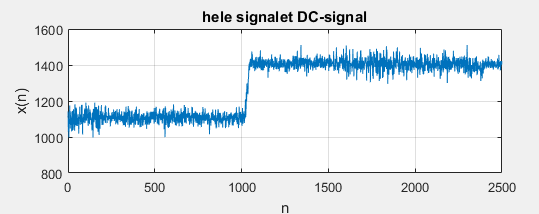
\includegraphics[width=0.8\textwidth]{rod/startsignal.png}
  \caption{hele signalet}
  \label{fig:helesignal}
\end{figure}

der ses på \ref{fig:helesignal} plottet af henholdsvist hele DC signalet, samt tidligere udregning af effektspektum, og et histogram plot lavet med histogram funktionen.
Der vurderes udfra disse effektspektre dette sagtens kan være normaltfordelt hvidstøj.
Ligeledes vurderes der de to middelværdier er henholdsvist 1100 samt 1400.

\subsection{afstand imellem bit niveauer i gram}
\label{sec:afstand}

\section{Design af midlingsfilter}
\label{sec:Design}

\subsection{påsætning af MA filter}
\label{sec:påsæt}

\begin{lstlisting}
%% MA-filter (ikke-rekursivt) variabler
M = 10;    % filterkoefficienter
hMA = 1/M*ones(1,M); % MA-filter, filterkoefficienter

hMA_imp_resp  = hMA;                        % impulsrespons
hMA_step_resp = filter(hMA,1,ones(1,2*M));  % steprespons
L_MA_trans_resp = M-1;                      % længde af transientrespons
HMA1 = fft(hMA,Nfft);                        % frekvensrespons

yMA1 = filter(hMA,1,x1);            % filtrerer inputsignal for første del
yMA2 = filter(hMA,1,x2);            % filtrerer inputsignal for anden del

var_x1 = var(x1(M:N1));    % varians i 1 signal i del efter transientrespons
var_yMA1 = var(yMA1(M:N1));% varians i 1 signal i del efter transientrespons

var_x2 = var(x2(M:N2));    % varians i 2 signal i del efter transientrespons
var_yMA2 = var(yMA2(M:N2));% varians i 2 signal i del efter transientrespons
\end{lstlisting}

følgende kode sætter filterkoefficienter op, udregner impulsrespons, stepresons, længde af transientrespons, frekvensrespons, samt lægger MA filteret på de to del signaler, og afslutningsvist udregner variansen ud med funktionen var, således dette kan plottes
variablen yMA1 samt yMA2 er vigtige, da disse skal anvendes til plotning af histogrammet efter filteret er påsat.
Der kan ses på koden der i første omgang er forsøgt at indsætte 10 filter koefficienter i koden her, plotsene med flere koeffecienter er ganske enkelt variablen M der er udskiftet med hvor end mange filterkoefficienter plotsene oplyses til at have.

\begin{lstlisting}
%% --- plotting for første MA filter signal ---
figure('name', 'første MA-filter')
subplot(2,6,1:3)
plot(n1,x1), grid
xlabel('n'), ylabel('x(n)'), title('første del af DC-signal')

subplot(2,6,4:6)
histogram(yMA1)
title('histogram')

subplot(2,6,7:10)
plot(n1,x1), grid, hold on
plot(n1,yMA1,'linewidth',2)
xlabel('n'), ylabel('x(n)'), title(['MA-filter, M = ' num2str(M)])
legend('input','output')

subplot(2,6,11:12)
text(0,0.5,...
    {['første MA-filter, M = ' num2str(M)],...
     ['Transientrespons: ' num2str(L_MA_trans_resp) ' samples'],...
     ['Støjeffekt i inputsignal (varians):  ' num2str(var_x1)],...
     ['Støjeffekt i outputsignal (varians): ' num2str(var_yMA1)],...
     ['Reduktion i støjeffekt: ' num2str((var_x1/var_yMA1)) ' gange'],...
     ['Reduktion i støjeffekt: ' num2str(10*log10(var_x1/var_yMA1)) ' dB']})
 axis off
\end{lstlisting}

følgende kode beskriver plotningen af MA filteret for første del, plotningen for anden del er identisk, og er derfor ikke beskrevet da den eneste forskel er N1 er udskfitet med N2, og ligeledes med x1 og x2.
første plot der sker viser del signalet der isoleret set er blevet kigget på, herefter plottes histogrammet med variablen yMA1 som i praksis er variablen der er blevet oprettet som konsekvens af påsætningen af filteret.
Herefter sammenlignes signalet før filteret blev udregnet med signalet efter, forhåbentligt skulle det gerne være fladet ud som efter filterets påvirkning.
afslutningsvist udregnes transientrespons, støjeffekt samt reduktion i støjeffekt i henholdsvist antal gange, samt i decibel.

\subsection{beregning af max FIR længde}
\label{sec:beregning}
\begin{figure}[h!]
  \centering
  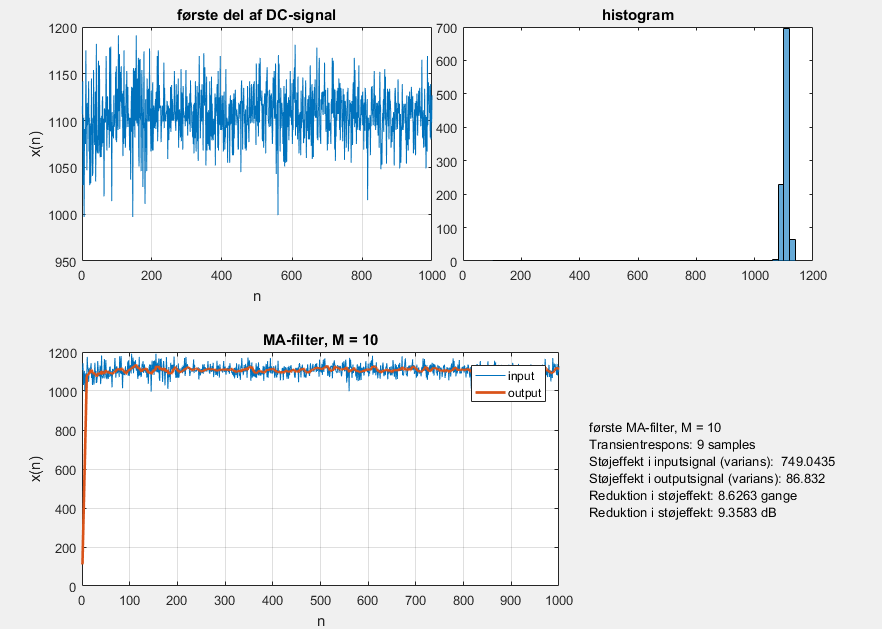
\includegraphics[width=0.8\textwidth]{rod/1MAfilter10.png}
  \caption{MA filter med 10 filter koefficienter}
  \label{fig:MA10}
\end{figure}

\begin{figure}[h!]
  \centering
  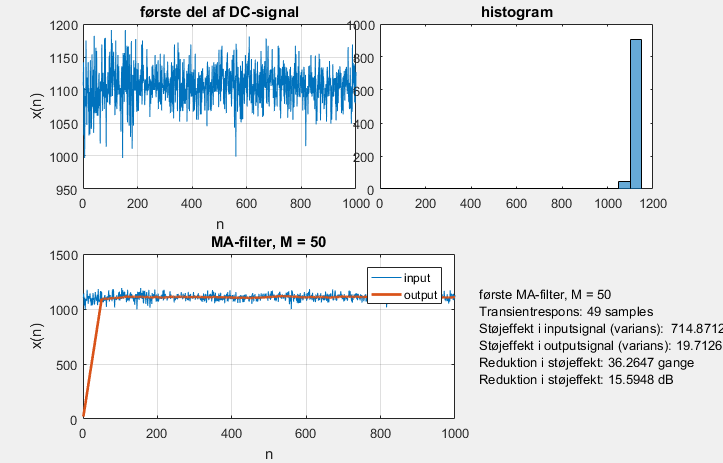
\includegraphics[width=0.8\textwidth]{rod/1MAfilter50.png}
  \caption{MA filter med 50 filter koefficienter}
  \label{fig:MA50}
\end{figure}

\begin{figure}[h!]
  \centering
  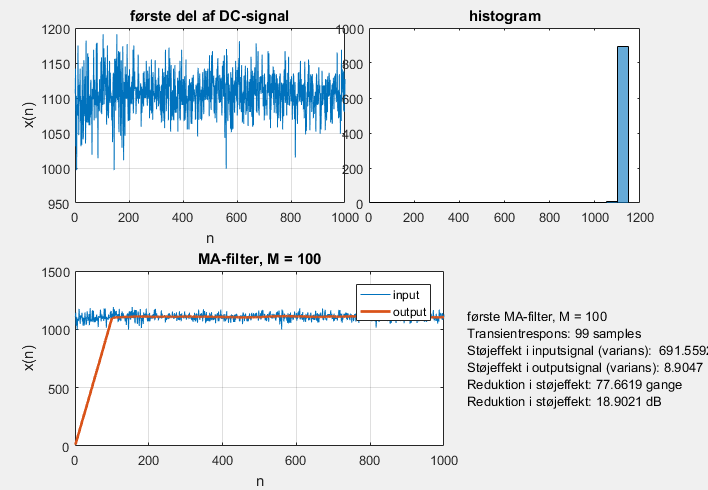
\includegraphics[width=0.8\textwidth]{rod/1MAfilter100.png}
  \caption{MA filter med 100 filter koefficienter}
  \label{fig:MA100}
\end{figure}

billede \ref{fig:MA10} \ref{fig:MA50} \ref{fig:MA100} viser de 3 MA filtre med henholdsvist 10, 50 og 100 filterkoefficienter, det der kan konstateres er reduktionen af støjeffekten bliver bedre, dæmpningen bliver bedre, men der går længere tid før outputtet giver respons da det tager fysisk længere tid for filteret at behandle signalet.
Altså variansen falder, når vi tager middelværdien af flere signaler, men indsvingningstiden stiger, så det er en priotering om hvad man vil have herfra.
Såfremt indsvingningstiden ville være på max 100 ms, ville det selfølgeligt afhænge af valgte samplingsfrekvens, den valgte i dette tilfælde er 300, så denne er hvad der udregnes med.

Der er taget udgangspunkt i tidligere givne formel for udregning på billede billede \ref{fig:formel}

\begin{figure}[h!]
  \centering
  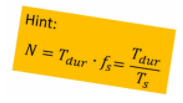
\includegraphics[width=0.2\textwidth]{rod/formel.png}
  \caption{formel for udregning af max antal MA-filtre}
  \label{fig:formel}
\end{figure}

\begin{figure}[h!]
  \centering
  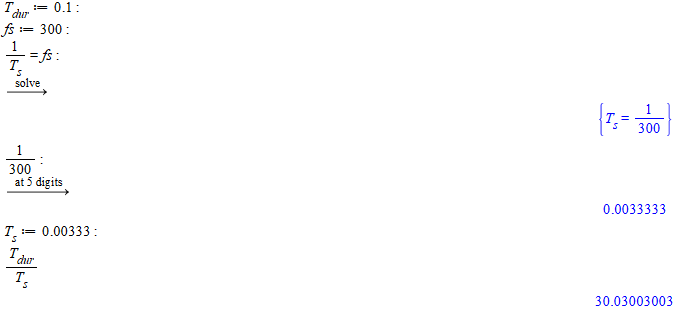
\includegraphics[width=0.8\textwidth]{rod/Max_udregning.png}
  \caption{max antal filtre}
  \label{fig:max_filtre}
\end{figure}

Der kan udfra dette konkluderes 30 ville være maximalt antal filterkoefficienter der ville kunne anvendes for at opnår ønskede indsvingningstid, dog med forbehold af fs er 300, såfremt denne ændres, ville max antal indsvingningstid ligeledes ændre sig.

\subsection{eksponentielt midlingsfilter}
\label{sec:eks}
\begin{lstlisting}
%% Eksponentielt midlingsfilter (rekursivt) variabler
alpha = 0.01;  % Lyons formel (11-31)

% b skabes da filter funktionen giver problemer med at filtere samme værdi
% 2 gange
b = alpha;
a = [1 -(1-alpha)];

hExp_imp_resp  = filter(b,a,[1 zeros(1,4*M-1)]); % impulsrespons
hExp_step_resp = filter(b,a,ones(1,4*M));        % steprespons

HExp1 = fft(b,N1)./fft(a,N1);                 % frekvensrespons
HExp2 = fft(b,N2)./fft(a,N2);                 % frekvensrespons

yExp1 = filter(b,a,x1);                      % filtrerer 1 inputsignal
yExp2 = filter(b,a,x2);                      % filtrerer 2 inputsignal

var_yExp1 = var(yExp1(M:N1));  % varians i signal i del efter transientrespons
var_yExp2 = var(yExp2(M:N2));  % varians i signal i del efter transientrespons

\end{lstlisting}

koden her viser til at starte med oprettelse af alfa variablen, denne er i eksemplet her sat til 0.01, koden er dog lavet på en måde således den er afhængig af denne variabel, og såfremt denne ændres til en andet ønsket værdi, reagerer koden herefter.
årsagen til variablen b skabes, er at ellers giver det fejl længere nede ved oprettelse af vExp1/vExp2 når filteret skal pålægges med filter funktionen såfremt dette skal foregå med samme variabel to gange i træk, eller når Hexp1/Hexp2 skaber frekvensresponset.
varians udregnes i de to del signaler afslutningsvist, og næste er at plotte.

\begin{lstlisting}
 %% plotting for første eksponentielle midlingsfilter (rekursivt) 
figure('name', 'Første eksponentielle midlingsfilter-filter')
subplot(3,1,1:2)
plot(n1,x1), grid, hold on
plot(n1,yExp1,'linewidth',2)
xlabel('n'), ylabel('x(n)')
title(['Eksponentielt midlingsfilter, \alpha = ' num2str(alpha)])
legend('input','output')

subplot(3,1,3)
text(0,0.5,...
    {['Eksponentielt midlingsfilter, \alpha = ' num2str(alpha)],...
     ['Støjeffekt i inputsignal (varians):  ' num2str(var_x1)],...
     ['Støjeffekt i outputsignal (varians): ' num2str(var_yExp1)],...
     ['Reduktion i støjeffekt: ' num2str((var_x1/var_yExp1)) ' gange'],...
     ['Reduktion i støjeffekt: ' num2str(10*log10(var_x1/var_yExp1)) ' dB']})
 axis off
\end{lstlisting}

samme approach som før er igen anvendt, hvor der kun redegøres for første del signal, da anden plot sektion igen er identisk bortset fra x1, n1 og yExp1.
første plot er det ikke filtreret signal, n1 over x1 i en plot funktion, denne bliver holdt således yExp1, som beskriver variansen i signalet efter pålagte filter, nu kan ses ovenpå.
Afslutningsvist plottes værdierne for støjeffekten i input samt output, og reduktionen i støjeffekt antal gange, samt i decibel plottes.


\subsection{Alfa's betydning}
\label{sec:alfa}

\begin{figure}[h!]
  \centering
  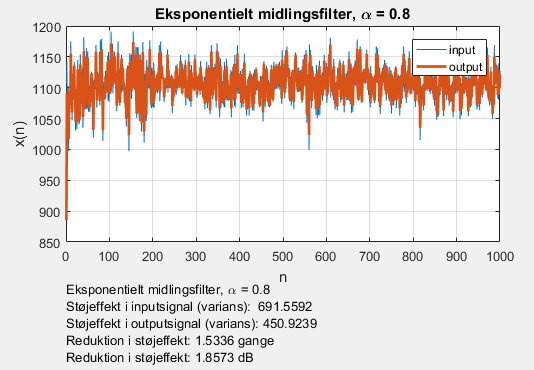
\includegraphics[width=0.8\textwidth]{rod/hoj_alfa.png}
  \caption{alfa på 0.8}
  \label{fig:høj_alfa}
\end{figure}

\begin{figure}[h!]
  \centering
  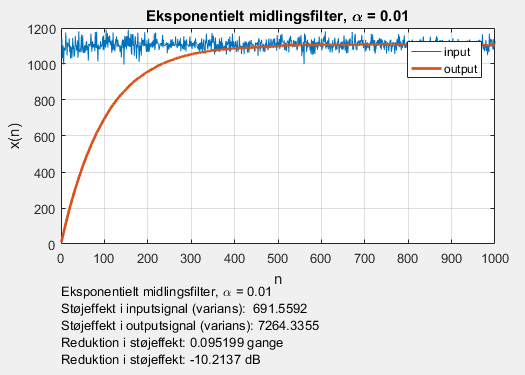
\includegraphics[width=0.8\textwidth]{rod/lav_alfa.png}
  \caption{alfa på 0.01}
  \label{fig:lav_alfa}
\end{figure}

som billede \ref{fig:høj_alfa} og \ref{fig:lav_alfa} illustrerer kan der ses at mindre alpha giver bedre dæmpning, men langsommere respons, og omvendt.

\subsection{ram samme værdi 100 filterkoefficienters MA filter}
\label{sec:ram}

\section{Systemovervejelser}
\label{sec:Systemovervejelser}

\end{document}
